\chapter{Trabajo 2 - SOC}

\note{\footnotesize Soy un estudiante italiano en Erasmus.
Hablo español bastante bien, pero me resulta más natural escribir en inglés; sin embargo, decidí escribir en español para practicar, con la ayuda de algunos traductores cuando era necesario. Si hay algo mal escrito o poco claro, estoy a disposición para cualquier aclaración.
}
\vspace{3em}

\framedt{Tarea a realizar}{

   \begin{itemize}
   \item Visualiza \href{
      https://www.bing.com/videos/search?q=security+operation+center+design&&view=detail&mid=FF7958286B4B6EBACA3CFF7958286B4B6EBACA3C&&FORM=VRDGAR&ru=\%2Fvideos\%2Fsearch\%3Fq\%3Dsecurity\%2Boperation\%2Bcenter\%2Bdesign\%26FORM\%3DHDRSC4}{este video}
	\item Identifica las funcionalidades que en el video se atribuyen a un SOC
	\item Para cada una de las funcionalidades definidas, indica que posibles herramientas de ciberinteligencia podrían implementar estas funcionalidades, de entre las herramientas analizadas tanto en las clases teóricas como en las prácticas de esta asignatura y asignaturas previas.
	\item ¿Consideras que alguna funcionalidad propia de un SOC no ha sido incluida en el vídeo? Indica cual o cuales. Puedes utilizar el documento adjunto como apoyo a tu respuesta.
\end{itemize}
\vspace{1em}
}
\vspace{3em}


\section{Introdución}

SOC significa Security Operations Center. 
La finalidad de un SOC es proteger la información de una organización, detectando y respondiendo a ciberataques.

\begin{definition}
   [SOC - Cyviz]
   The fundamental aspects of an effective SOC is the ability to examine and \textbf{analyze} big and sensitive data flows, and to \textbf{correlate}
other incidents from a cybersecurity perception. Security operations teams need \ul{appropriate tools and techniques to process,
visualize and correlate} the enormous amount of historical and real-time data.
\end{definition}

\subsection{Costruir un SOC}
Como arquitectos de seguridad, para construir un SOC, necesitamos ante todo {\textbf{identificar} cuales son los datos que vamos a recoger, y con cual frequencia vamos a recogerlos}, cuántos eventos por segundo/minuto/hora y cuánto storage necesitaremos.\\
Después, tenemos que decidir dónde colocar los sensores (collectors) de esos datos.\\
Al final, deberiamos diseñar e implementar una User Interface para los analistas, que les permita visualizar los datos y tomar decisiones.

Es fundamental identificar {cuales son los \textit{crown jewels} de la organización}, y protegerlos con mayor prioridad, gestionándolos lo más rápidamente posible.

\coolquote{
   A \textbf{crown jewel} one of the highest-value assets in your industrial control systems (ICS) and operational technology (OT) environment that, if compromised, could cause major impact to the organization 
}{\href{https://www.dragos.com/blog/how-to-identify-cyber-critical-systems-with-a-crown-jewel-analysis/}{dragos.com}}

% \newpage
\section{Funcionalidades más importantes de un SOC}


{Las funcionalidades cruciales mencionadas en el vídeo que el SOC debe implementar, son las siguientes:\ns
\begin{enumerate}
   \item \ul{\textbf{Agregar} datos}
   \item \ul{\textbf{Normalizar} datos}, para que los analistas puedan escribir detecciones y reglas a partir de los datos
   \item \ul{\textbf{Personalizar las detecciones}}, adaptarlas a la estructura y las necesidades de la organización, para limitar el riesgo de falsos positivos y comprender la criticidad de un incidente en relación con el contexto de la organización.
   \item \ul{\textbf{Proteger} datos sensibles}, según un criterio de priorización.
   \item\ul{\textbf{Automated responses}}. Es importante minimizar el tiempo de remediación, utilizando modernas herramientas que permitan automatizar la respuesta a los eventos, en lugar de enviar una alerta a un servicio de tickets, abrir un ticket, asignarlo a un analista, etc. 
\end{enumerate}
}

Estas funcionalidades coinciden con los mencionados en el artículo de Cyviz, aunque organizados de forma ligeramente diferente.
El artículo propone \textit{``Identify'',} \textit{``Protect'',} \textit{``Detect''} and \textit{``Respond''} como puntos clave, pero el significado es más o menos el mismo.


En el video también se menciona la importancia de \textbf{monitorizar} constantemente el estado del SOC y de los sensores, para asegurarse de que está funcionando correctamente, evaluar disponibilidad y scalabilidad y si son apropriadas nuevas tecnologías, herramientas, dispositivos.


Vamos a ver cómo se pueden implementar estas funcionalidades con las herramientas que hemos visto en clase.
\subsection{Agregar, normalizar datos y personalizar detecciones}

% \begin{paracol}{2}
%    Hemos visto cómo la Ciberconciencia Situacional se construye a partir de las fuentes de la ciberinteligencia.\\
%    Hay muchas posibilidades
   
%    \switchcolumn

%    \begin{figure}[htbp]
%       \centering
%       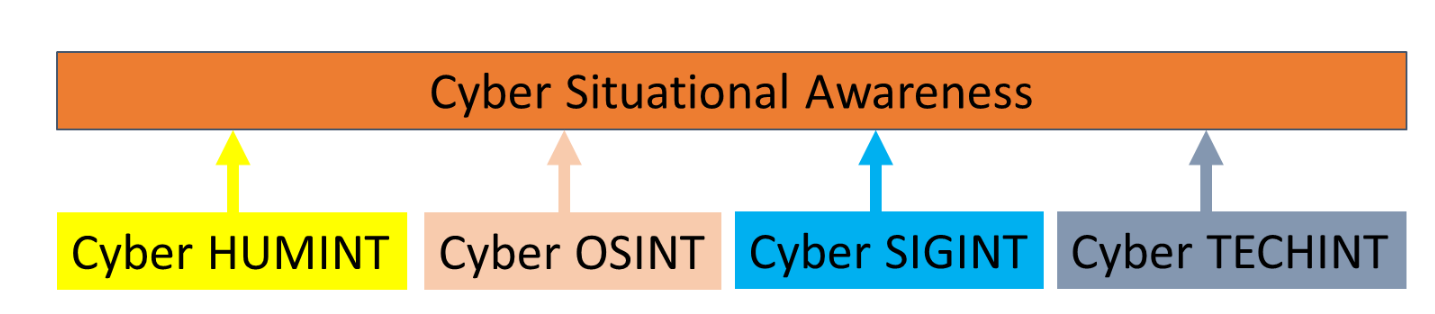
\includegraphics{images/cybersit.png}
%       % \caption{}
%       \label{fig:cybersit}
%    \end{figure}
% \end{paracol}

Antes de agregar datos, es necesario recorgelos, pero las herramientas para hacer esto no están tratadas en el video o en el artículo, que, en cambio, apuntan a la atención que debe prestarse en general al diseño de la recogida de datos, sin entrar en detalles de implementación.\\
Hay muchas herramientas y sensores que pueden ser fuentes de datos, por ejemplo NIDSs/HIDSs (\textsl{OSSEC}, \textsl{Snort}, \textsl{Suricata}, \dots), firewalls, network monitoring tools (\textsl{Zeek},\dots), EDR tools,\dots
\note{En la practica de la semana pasada hemos utilizado SELKS, que es un IDS/IPS. Incluye, entre otros, Suricata y Kibana.}

\begin{paracol}{2}
   \colfill
   Es más interesante cómo \ul{\textbf{agregar}} datos de diferentes fuentes, y por esto existen los \textsc{SIEM}s, que hemos visto en clase.\\
   El objetivo de un \textsc{SIEM} es analizar registros y correlacionar eventos para detectar patterns que indiquen ataques, y tipicamente son asignados a subredes o partes de subredes.

   Un \textsc{SIEM} muy utilizado es \textsc{Splunk}, pero hay otros, como \textsc{QRadar}, \textsc{OSSIMO}, o \textsc{AlienVault}, que pero es más viejo.
   
   Algunos \textsc{SIEM}s también ofrecen la posibilidad de integrar información sobre el contexto de la organización, como la estructura de la red, las vulnerabilidades, cuales son los \textit{crown jewels} de la organización, o asignar assets a business functions, \ul{\textbf{personalizando}} el proceso de detección.\\
   En esta manera, la severidad de un evento puede ser evaluada en relación con el contexto de la organización.
   \colfill

   \switchcolumn

   \begin{figure}[htbp]
      \centering
      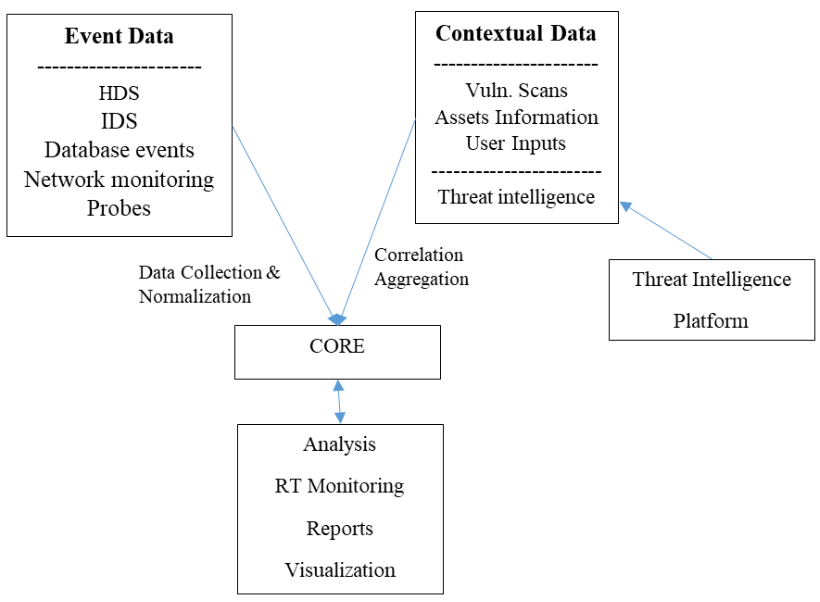
\includegraphics[width=0.9\columnwidth]{images/siem.png}
      \caption{\textsc{SIEM} architecture}
      \label{fig:SIEM}
   \end{figure}
\end{paracol}

El \textsc{SIEM} permite ``to flatten raw data'', y por tanto de \ul{\textbf{normalizar}}, para salir una alerta más concisa y relevante.\\
En el video con ``normalizar'' se entiende también hacer que los datos sean \textbf{visibles} para los analistas, y en este sentido hemos visto en clase diversas técnicas de \textbf{visualización}, que permiten de ver las relaciones entre los elementos.\\
La tipología de visualización depende de los datos que se quieren representar, y de la finalidad de la visualización.
% \newpage
\begin{paracol}{2}
   

   \begin{figure}[htbp]
      \centering
      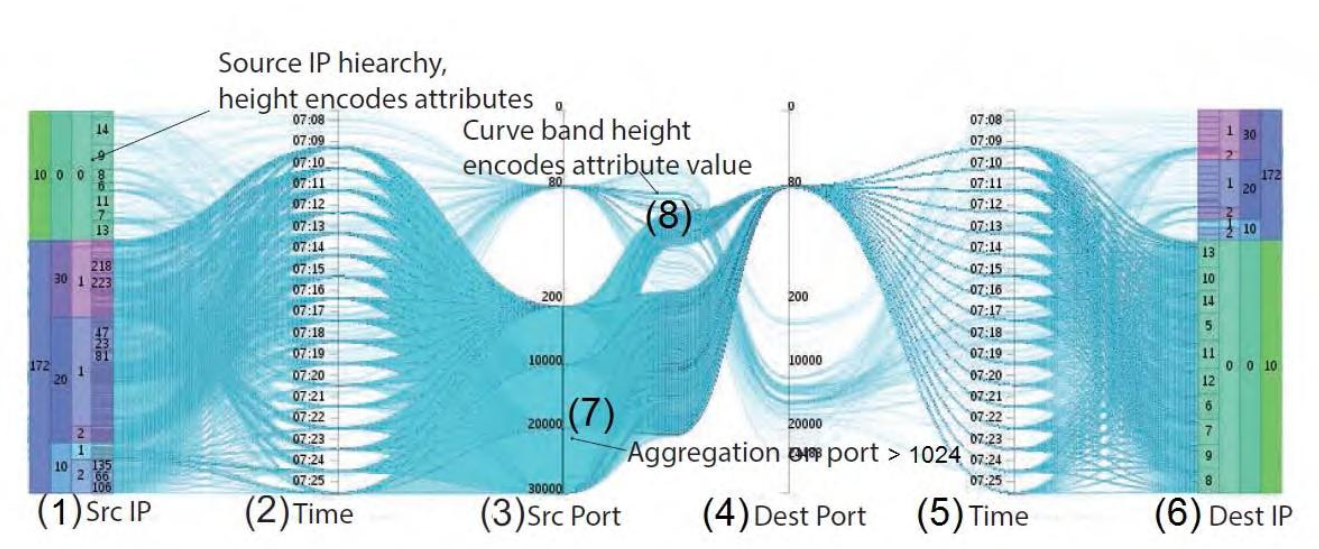
\includegraphics[width=0.75\columnwidth]{images/chart.png}
      \caption{Connections flow chart}
      \label{fig:chart}
   \end{figure}

   \switchcolumn
   \colfill
   Lo más intuitivos son grafos, pero no siempre son suficientes para representar la complejidad de las relaciones entre los datos, porque los grafos tienen solo dos dimensiones (se pueden añadir más, utilizando el color o el tamaño de los nodos, sin embargo son limitadas en algunos casos).\\
   En Fig. \ref{fig:chart} se puede ver un ejemplo de un diagrama de flujo de conexiones, que permite de identificar rápidamente horizontal/vertical port scanning o DDoS ataques.
   \colfill
\end{paracol}

\newpage
\subsubsection{Herramientas de visualización}
\begin{figure}[htbp]
   \centering
   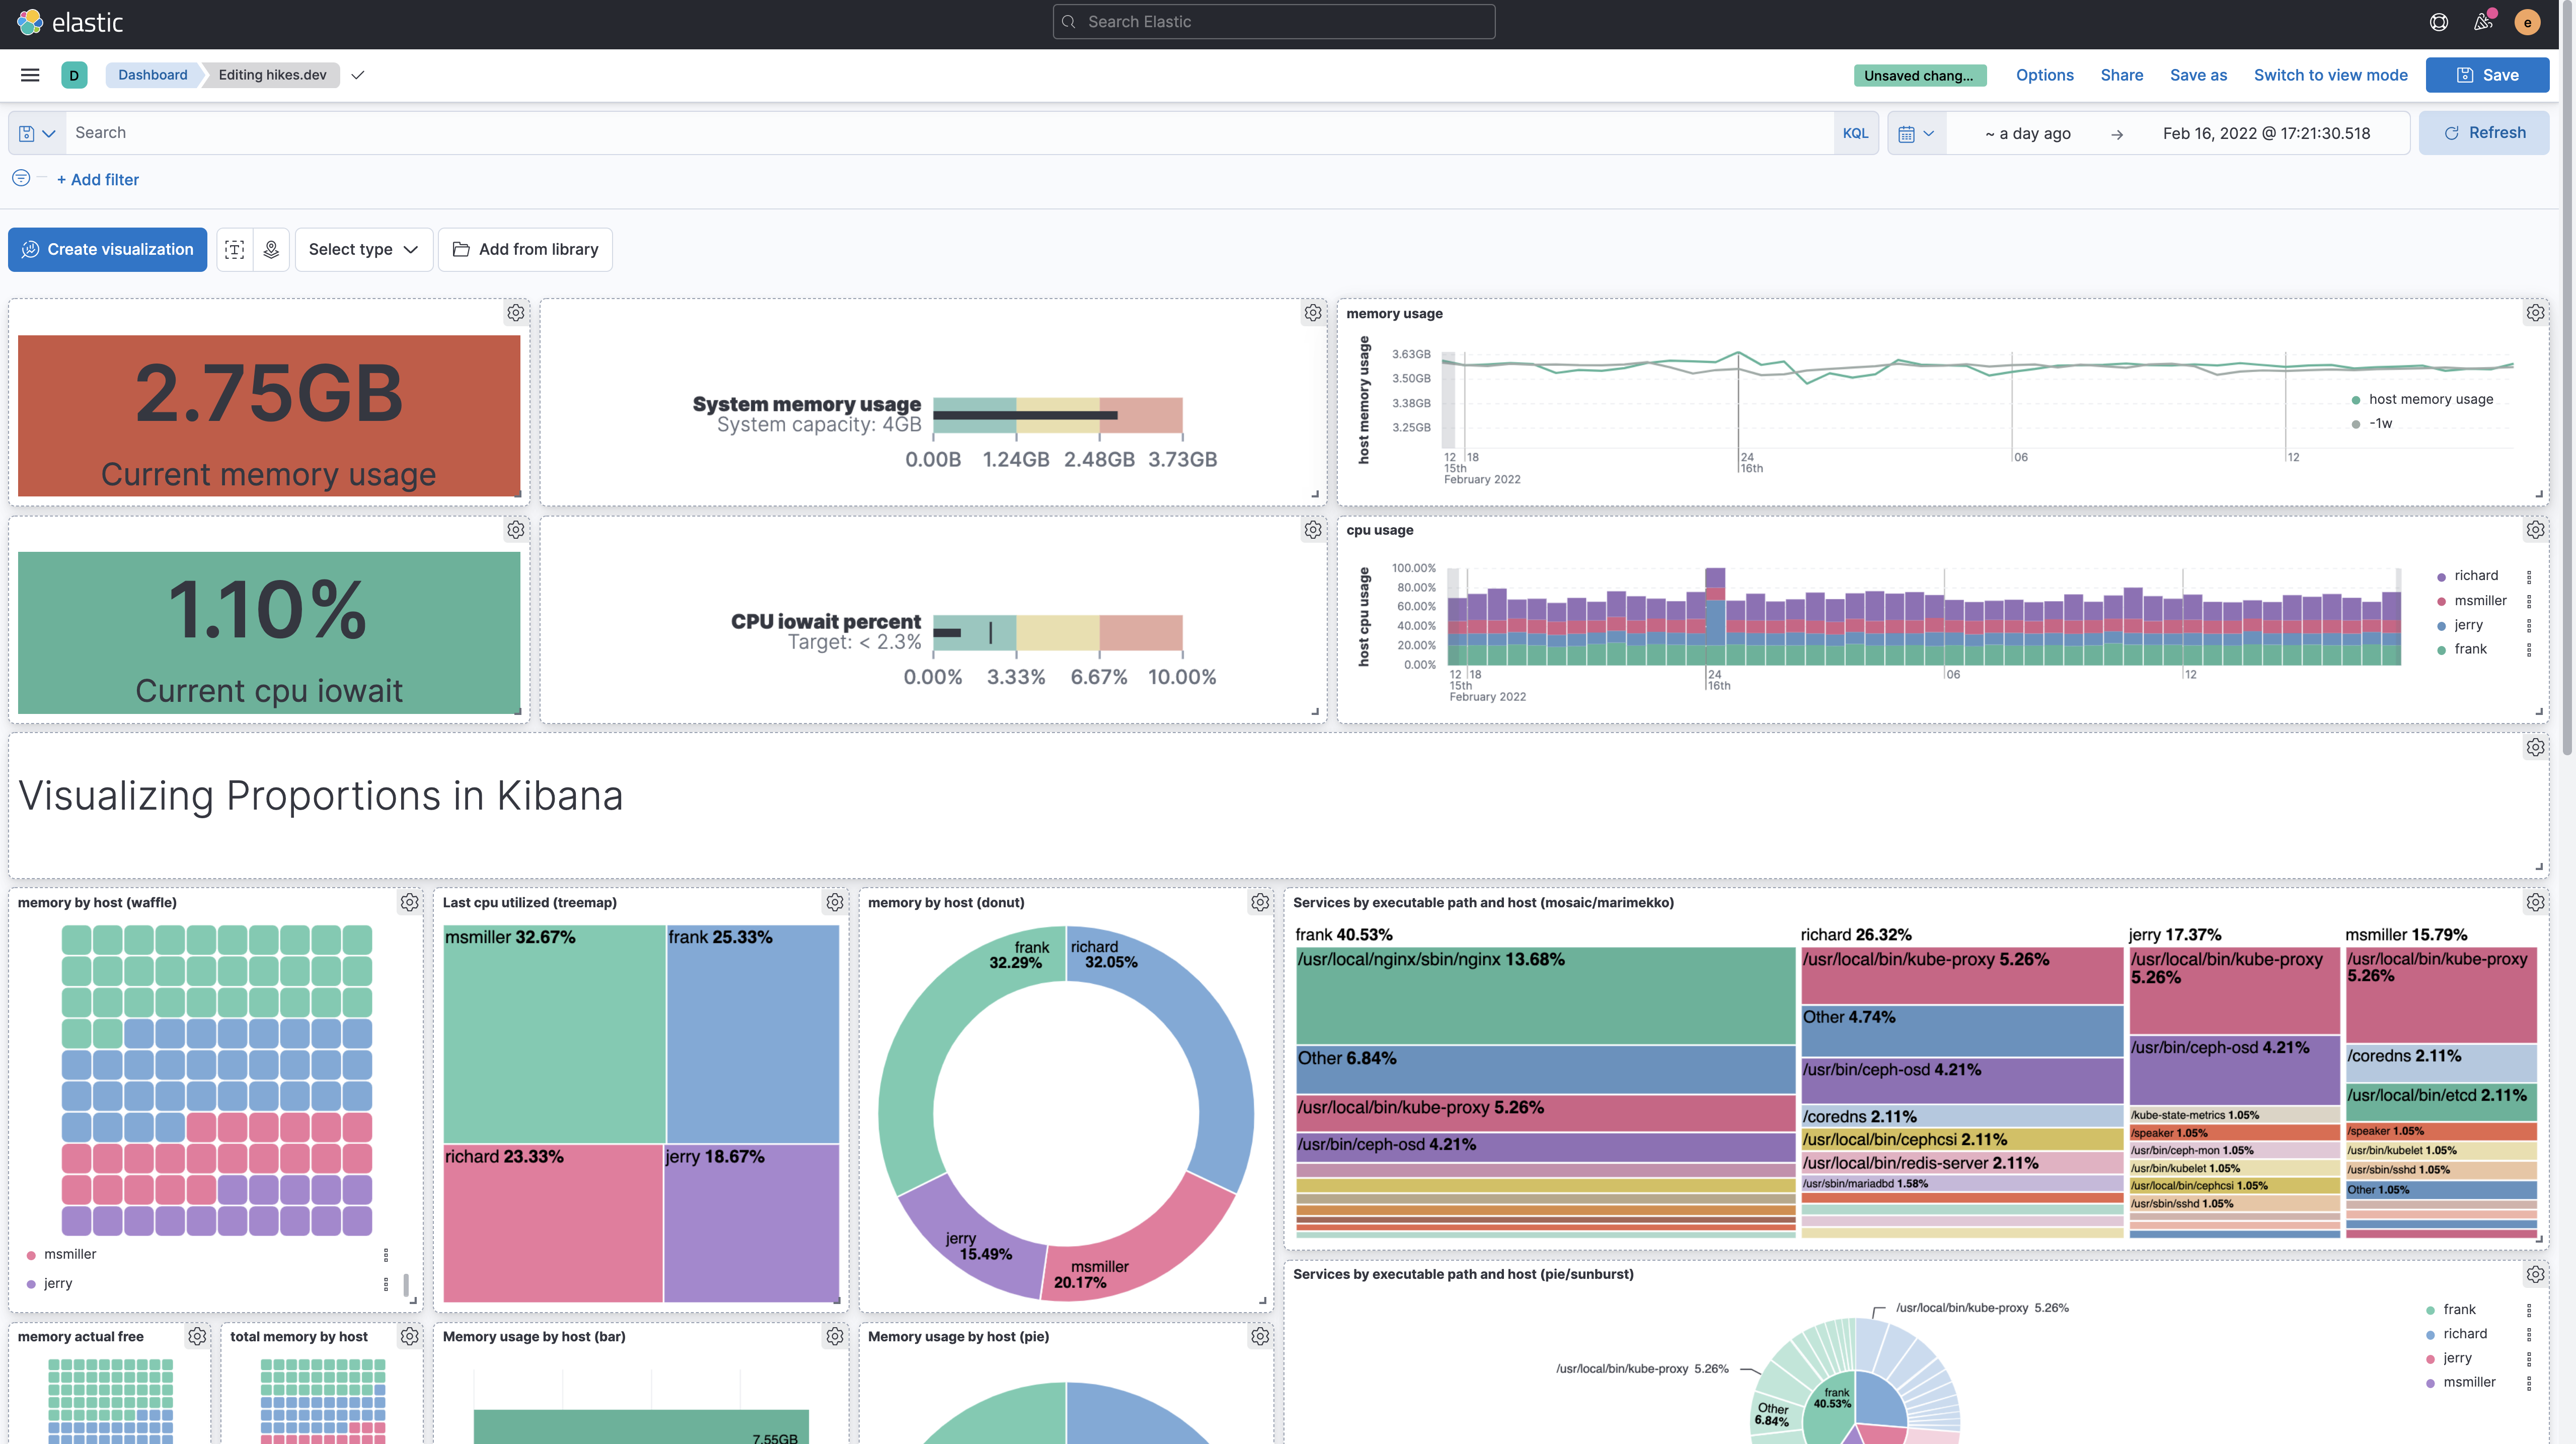
\includegraphics[width=0.49\columnwidth]{images/kibana.png}
   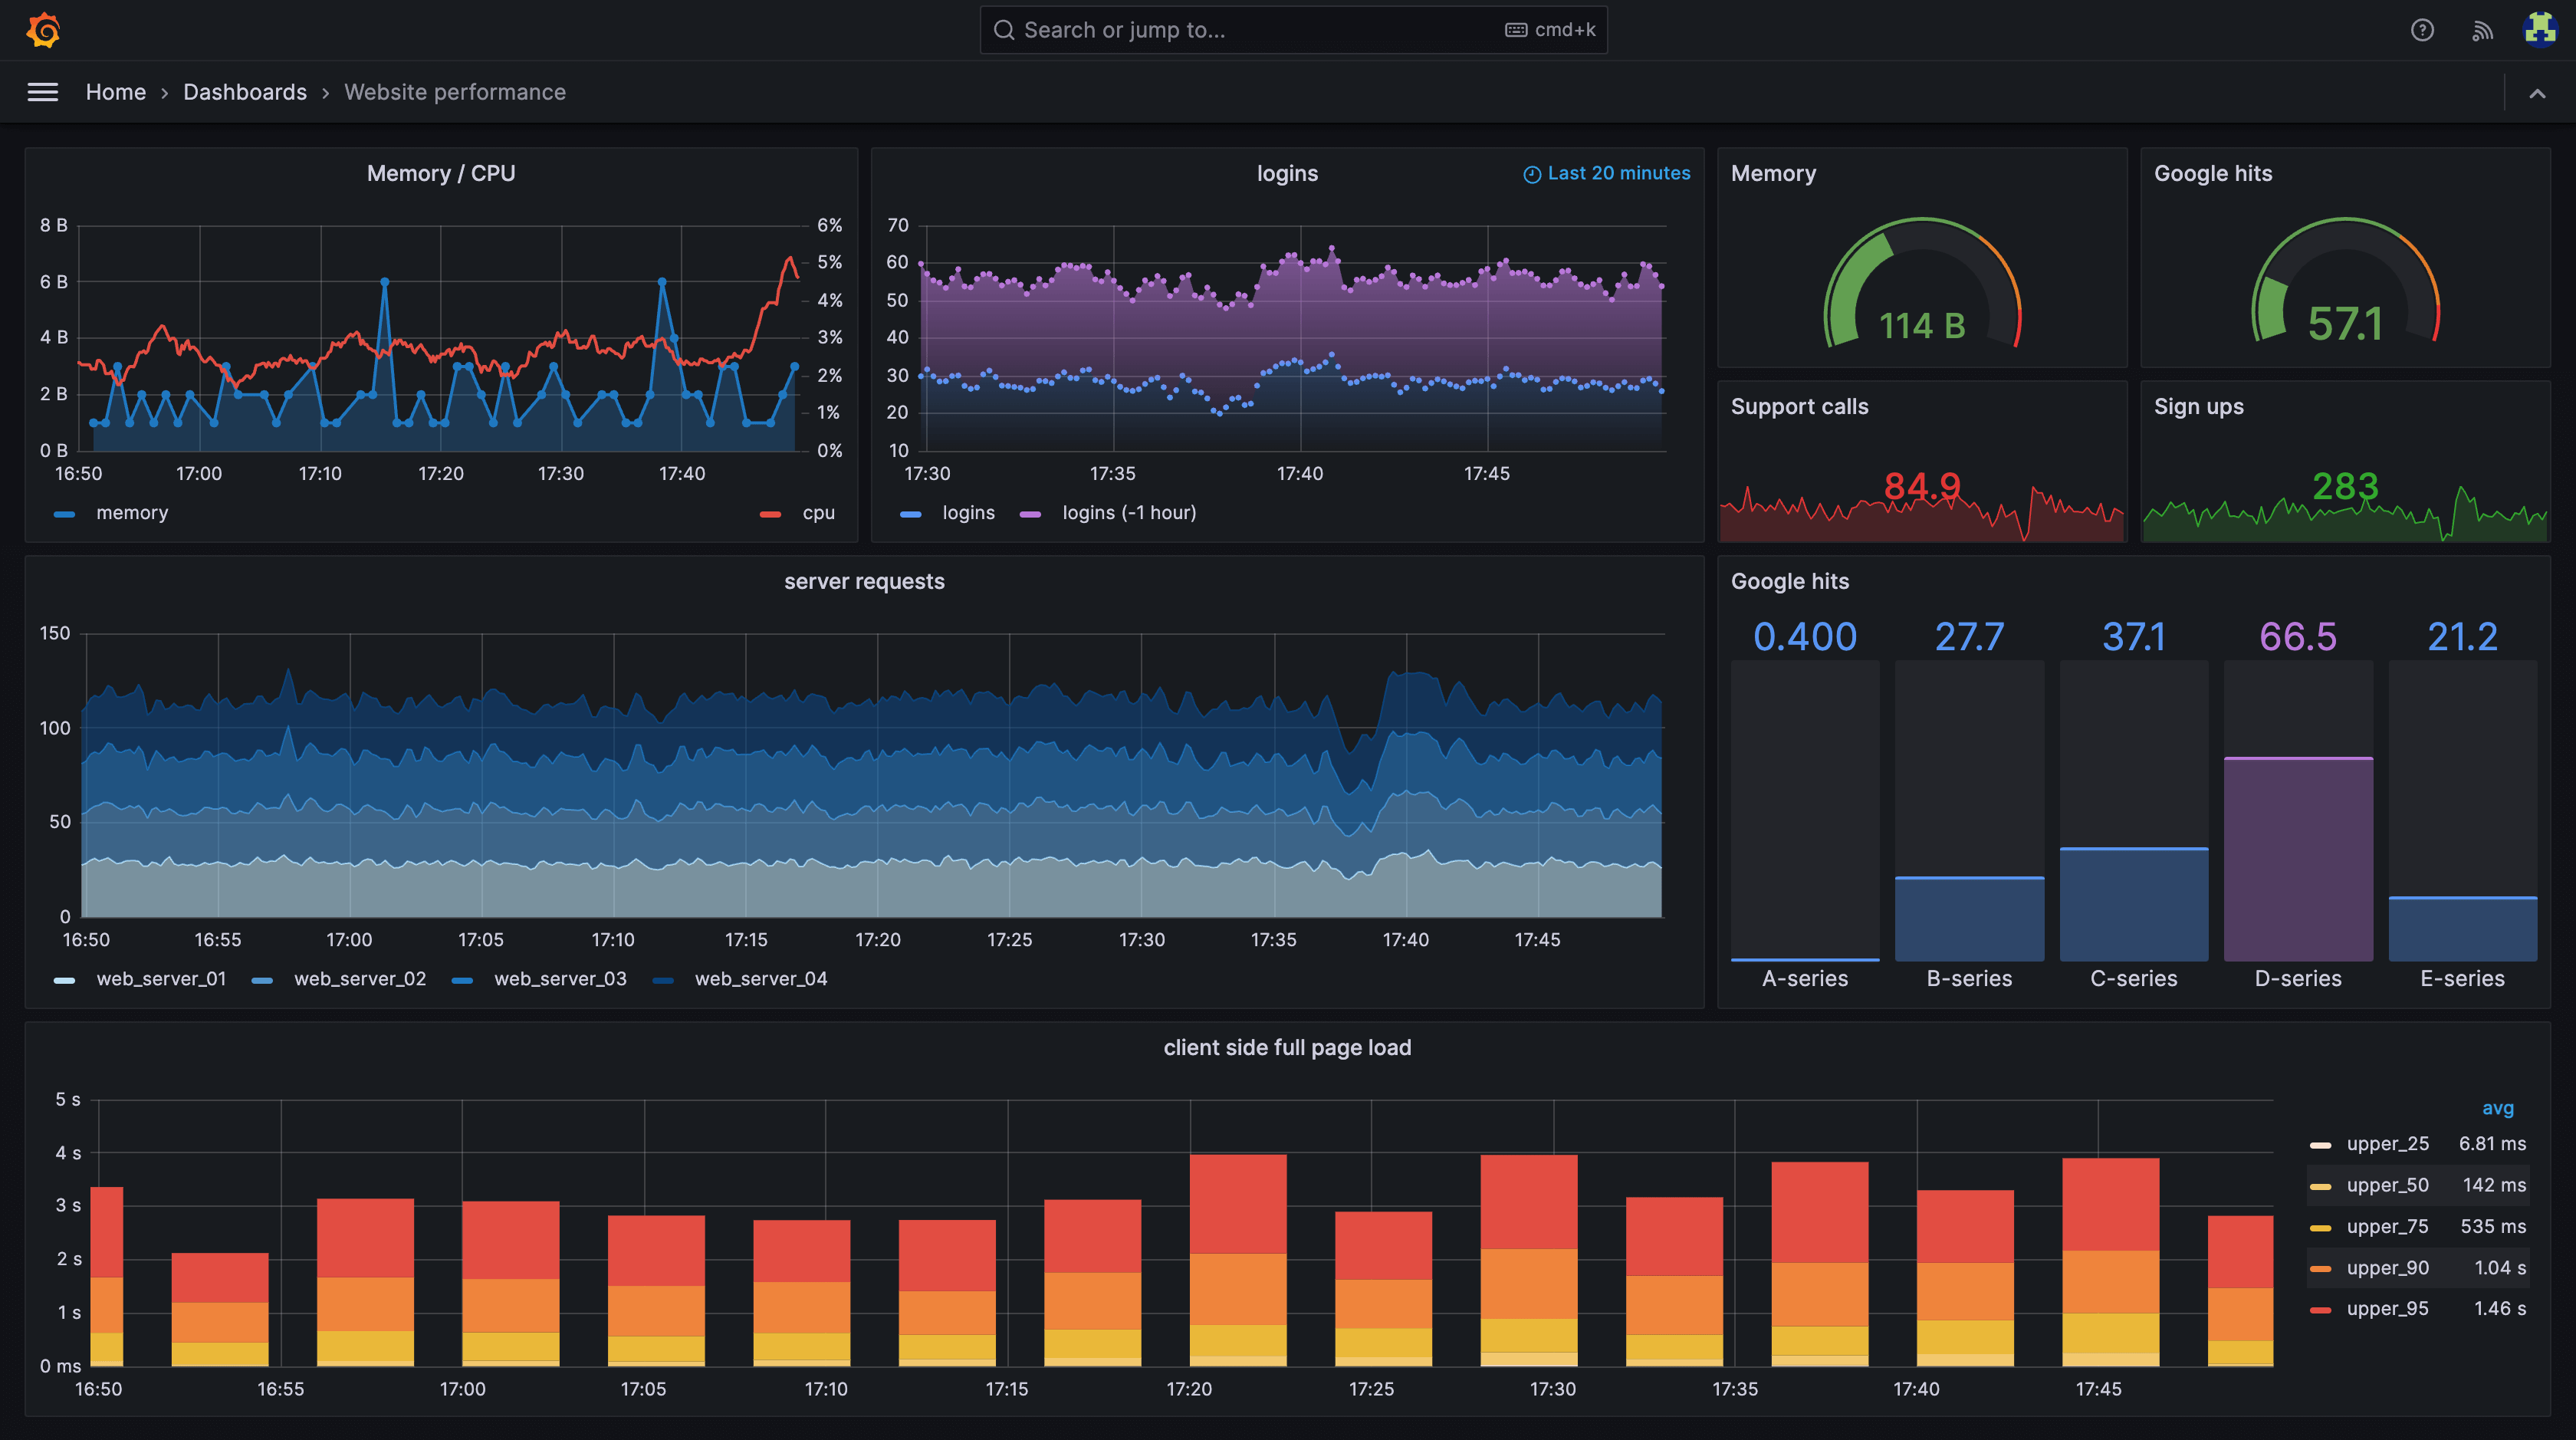
\includegraphics[width=0.49\columnwidth]{images/grafana.png}
   \caption{\textsc{Kibana} y \textsc{Grafana}}
   \label{fig:kibana}

   \textsc{Kibana} ofrece muchos tipos de gráficos diferentes, también algunos que no se muestran en la figura, como heatmaps y geomaps. \textsc{Grafana} es otra herramienta de visualización popular, que se centra más en los datos de series temporales, y también ofrece una amplia gama de opciones de visualización. 
\end{figure}

\begin{figure}[htbp]
   \centering
   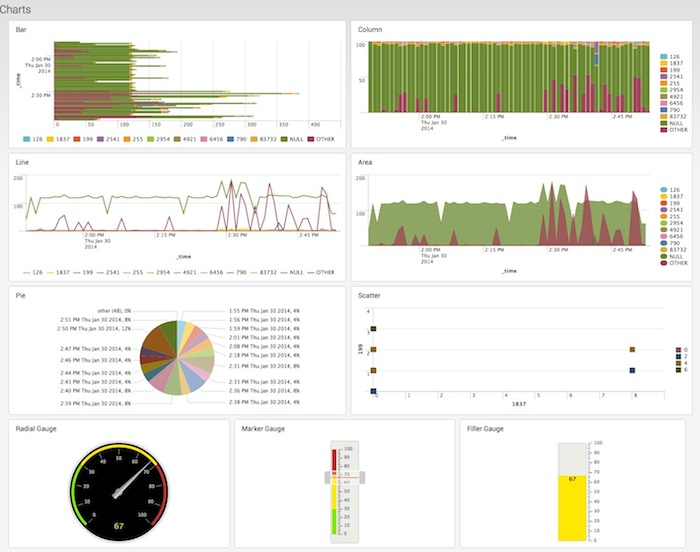
\includegraphics[width=0.49\columnwidth]{images/splunk.jpg}
   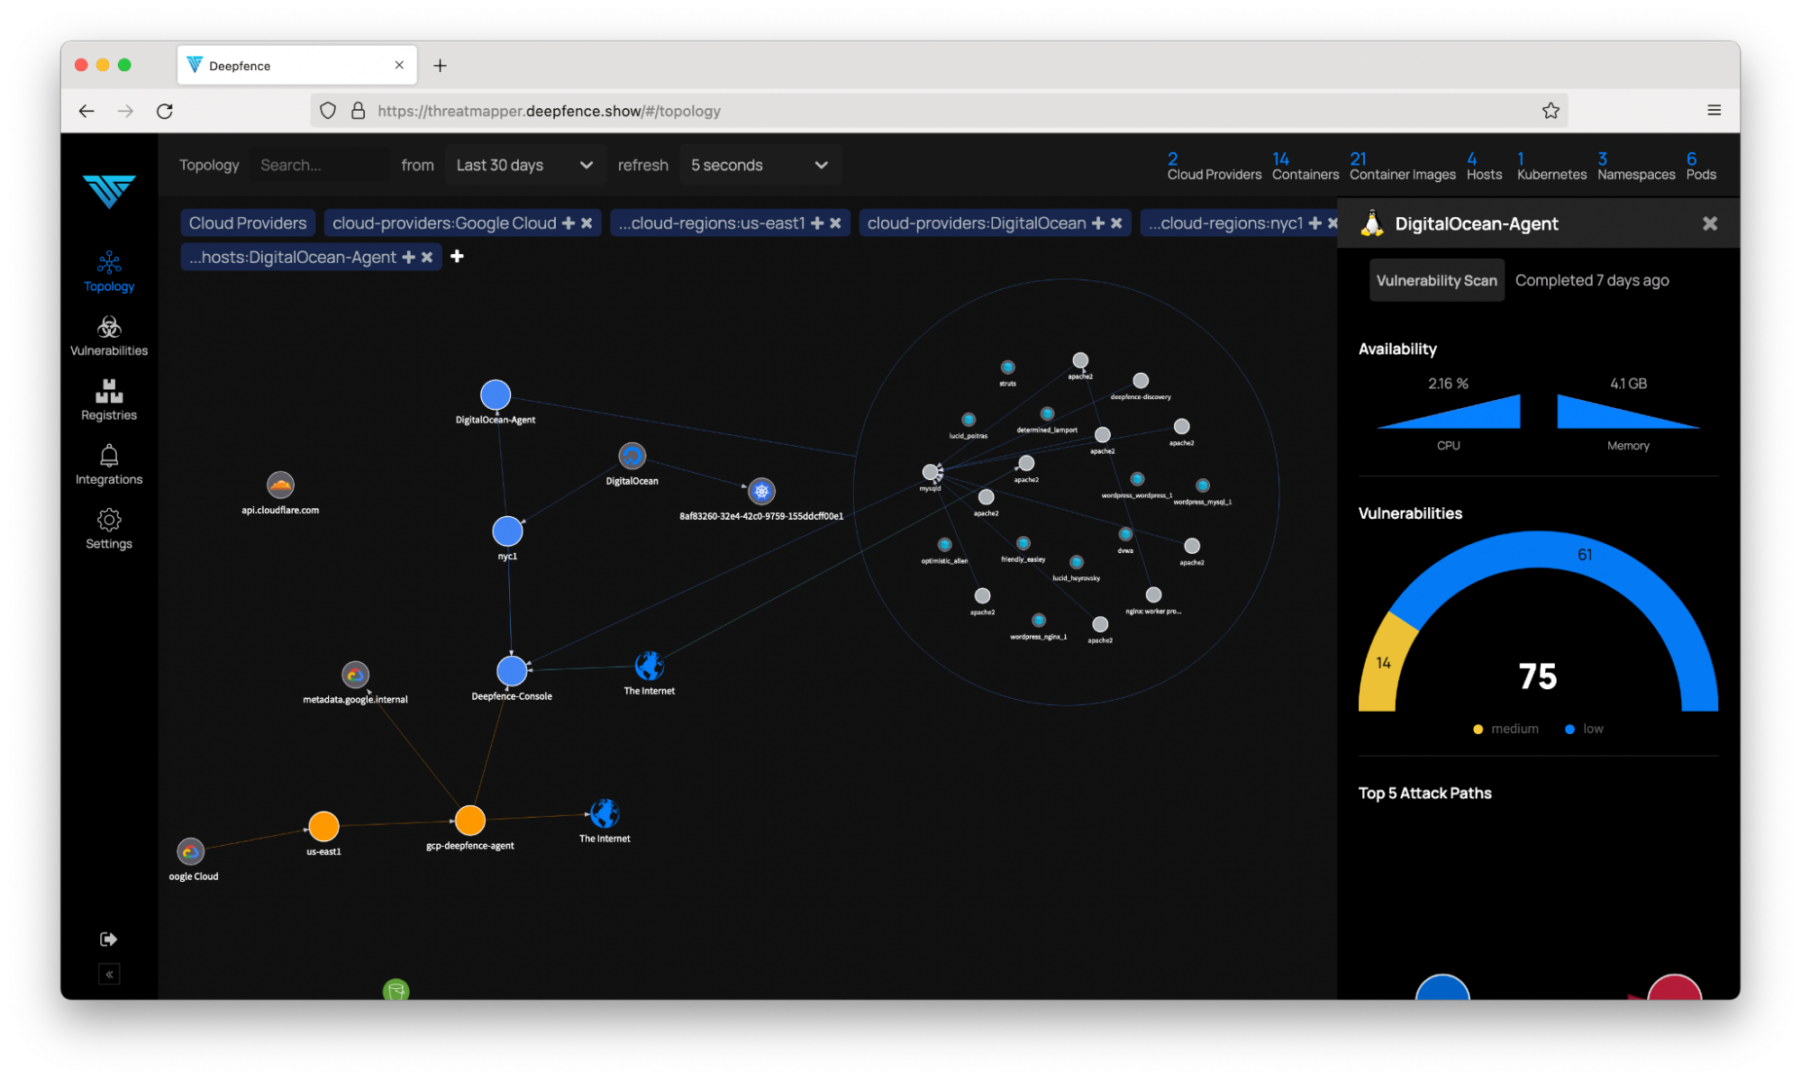
\includegraphics[width=0.49\columnwidth]{images/threatmapper.png}
   \caption{\textsc{Splunk} and \textsc{Threatmapper}}
   \label{fig:splunk}
   Las capacidades de visualización de \textsc{Splunk} se integran con el resto de la plataforma, y es posible crear cuadros de mando personalizados. \textsc{Threatmapper} es una herramienta que permite visualizar la superficie de ataque de una organización, y también mostrar rutas de ataque, que representan los pasos que daría un atacante para alcanzar un objetivo.
\end{figure}

\subsection{Proteger datos y Automated responses}

Claro que la \ul{\textbf{protección}} de los datos es una de las funcionalidades más importantes de un SOC, y es necesario proteger los datos más sensibles con mayor prioridad.\\
Gracias a los sistemas de detección y visualización, los analistas pueden identificar rápidamente las amenazas y responder adecuadamente, apoyándose posiblemente en procedimientos de remediación ya escritos y documentados. 
A menudo conviene integrar estos procedimientos con los standards que clasifican las vulnerabilidades y amenazas, como el \textsc{MITRE ATT\&CK Framework}, \textsc{CVSS}, \textsc{CVE}, \textsc{STIX}, que hemos mencionado en clase. 

Sin embargo, para velocizar el proceso de remediación, es posible \ul{\textbf{automatizar}} las respuestas a los eventos, utilizando herramientas como \textsc{SOAR}, que tal vez se pueden integrar con el \textsc{SIEM}.\\
El orador del vídeo presenta este aspecto como uno de los más importantes, porque minimizar el tiempo de remediación es fundamental para limitar el daño de un ataque.
Él introduce en la entrevista el concepto de \textbf{playbook} (más sobre esto más abajo), que define una secuencia de acciones que deben ser ejecutadas para realizar un objetivo, y que pueden automatizarse.



% \subsection{Tratamiento de los falsos positivos}
% \coolquote{
%    Como tratar el enorme número de falsos positivos?
% }{}
% Una manera es considerar como un un ataque con éxito parece al analista.\\
% Por ejemplo, si despues de una alierta de port scanning no hay tráfico permitido, no es necesario esaminarlo.\\
% Con una métrica de ``fidelity'', podemos reducir la tasa de verdaderos/falsos positivos.

% \subsection{Monitoring SIM and SOC}
% Despues de diseñar y implementar un SIM (Security Information Management), es necesario \textbf{monitorizar} su ``health'' en el día a día, para asegurarse de que está funcionando correctamente, y que la nuestra solución SOC funciona correctamente también.\\
% En particular, es necesario evaluar la disponibilidad y escalabilidad, y si nuevas tecnologías y herramientas pueden ser integradas en el sistema.

% SIM se considera la herramienta para detectar, pero luego la respuesta depende de SOC.
% Así que es importante escribir hasta 20 o 30 ---automatizable--- \textbf{playbooks} diferentes, para responder a diferentes tipos de ataques, y luego también tienes \textbf{runbooks} (también llamados SOP, \textit{Standard Operating Procedures}) para responder a diferentes tipos de alertas.\\
% Los runbooks definen las acciones de alto nivel que deben emprenderse en respuesta a una alerta, y los playbooks definen las acciones reales que deben emprenderse, \ul{y generalmente son \textbf{automatizados}}.
% \begin{align*}
%    \textit{Runbook} &\longrightarrow \textit{Statements}\\
%    \textit{Playbook} &\longrightarrow \textit{Actions}
% \end{align*}
% \framedt{Example - Machine got compromised}{
%    A Machine got compromised, and the runbook says that the scenario must be assessed (what did user do, when, if there's a ransomware\dots) and that the machine must be isolated from the network. 
%    While, in the playbook there is written how to actually isolate the machine from the network.
% }


% \subsection{Integrating Cloud}
% El último tema mencionado se refiere a la integración de la nube en el entorno SOC.\\
% Es importante la visibilidad y las regulations laws, para saber que datos se pueden recoger y almacenar en la nube, si son masked o unmasked.
% Es importante también considerar que utilizar la nube puede ser limitante, porque depende de un proveedor externo para la funcionalidad de los servicios.

\newpage
\section{Diferencias entre el video y el artículo}
\begin{paracol}{2}
   

   \begin{figure}[htbp]
      \centering
      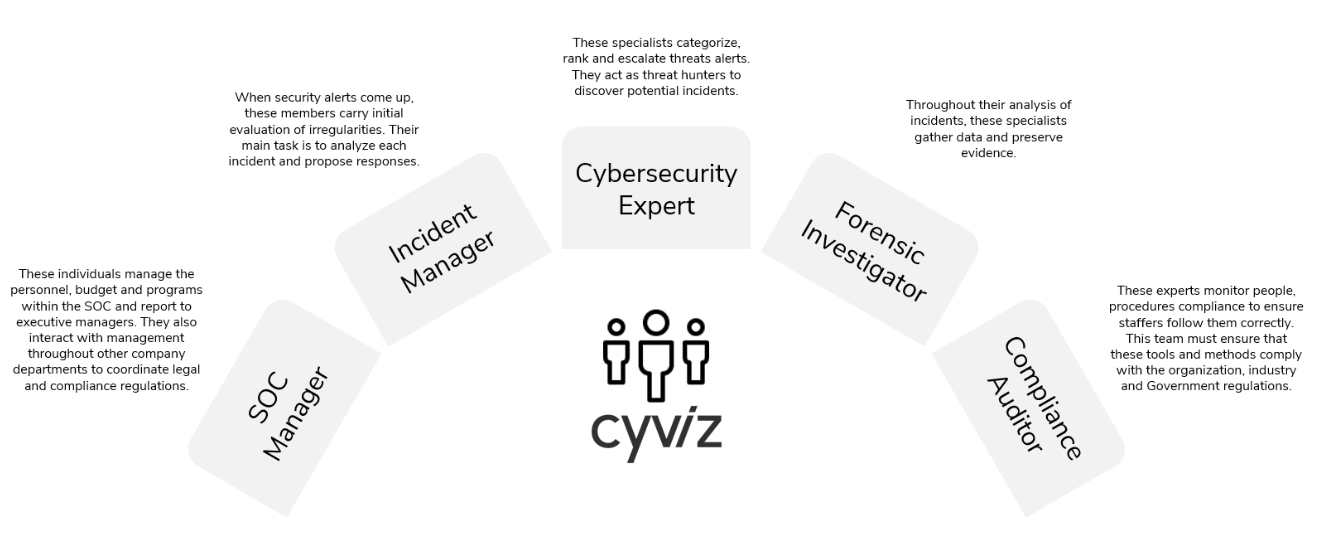
\includegraphics[width=0.95\columnwidth]{images/cyvizTeam.png}
      \caption{Propuesta de organización del equipo Cyviz}
      \label{fig:cyvizTeam}
   \end{figure}
   \switchcolumn
   \colfill
   En el artículo hay algunas secciones sobre la estructura y la finalidad de los \textbf{equipos de seguridad}, que no se exploran en profundidad en el vídeo, que se centra más en los SOC desde el punto de vista de la arquitectura y el diseño.\\
   También hay algunas menciones relativas a los diferentes modelos operativos del SOC, si debería ser \textit{Internal}, \textit{Virtual}, \textit{Outsourced}, \dots
   \colfill
\end{paracol}

Aunque estos aspectos no se tratan en profundidad en el vídeo, algunos se mencionan brevemente, lo que me hace pensar que el orador es consciente de ellos, pero no son el centro de la entrevista.\\
Por ejemplo, en el artículo se puede leer:
\begin{center}
   \textit{``An incident response team is crucial to building a functional SOC. It can decide the best way to assign and manage incidents, and
   act on a defined action plan. They also establish a repeatable workflow and craft essential communication between the business,
   legal and PR teams. They need to strictly follow a predefined response plan and/or craft new plans to address new scenarios and
   unknown threats''}
\end{center}

En el video se habla de la importancia de \textbf{runbooks} y \textbf{playbooks}, y que son fundamentales ---aparte de su uso principal de automatizar las respuestas--- para definir workflows repetibles que puedan enseñarse fácilmente a los nuevos miembros del equipo.

\note{Los \textbf{runbooks} definen las acciones de alto nivel que deben emprenderse en respuesta a una alerta, y los \textbf{playbooks} definen las acciones reales que deben emprenderse, \ul{y generalmente son \textbf{automatizados}}.
\begin{align*}
   \textit{Runbook} &\longrightarrow \textit{Statements}\\
   \textit{Playbook} &\longrightarrow \textit{Actions}
\end{align*}
Por ejemplo, en caso de que un dispositivo se viera comprometido, el runbook diría que hay que evaluar el escenario (qué hizo el usuario, cuándo, si hay un ransomware\dots) y que hay que aislar el dispositivo de la red.
Mientras que en el playbook está escrito cómo aislar realmente en practica el dispositivo de la red.
}
\nl

Y con respecto a la Fig. \ref{fig:cyvizTeam}, el orador no habla de esos ``equipos dedicados'', sino que menciona las actividades que realizan, como la categorización de alertas, la investigación de una alerta o el análisis retrospectivo de un incidente, y es razonable pensar que estas actividades se dividen y se asignan a diferentes equipos con diferentes funciones y permisos, aunque no se menciona explícitamente.